\section{Parsing}
\begin{frame}
    \begin{block}{What's a parser?}
        Part of the compiler.
        Checks the stream of tokens produced by the \emph{lexer} for syntactical errors
        and produces an IR representation (usually an abstract syntax tree) of the source 
        that is used in later steps to generate machine code.
    \end{block}
    \begin{figure}
        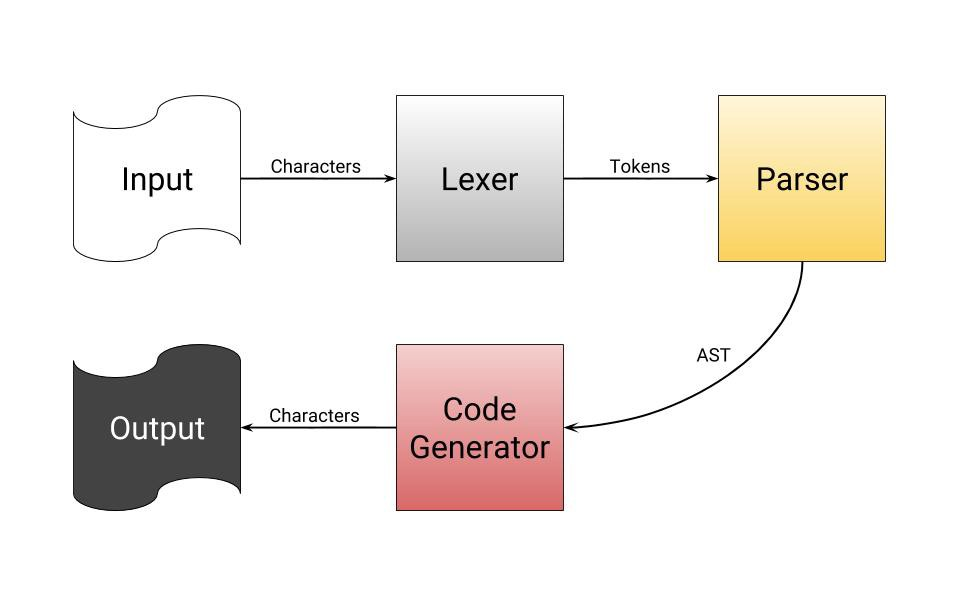
\includegraphics[width=\textwidth]{img/parser.jpg}
    \end{figure}
\end{frame}
\begin{frame}
    \frametitle{Context free grammars}
    
    \begin{block}{}We need a model to describe a language syntax.\end{block}
    \pause
    \begin{block}{}Classical problem, solved by using formal language theory.\end{block}
    \pause
    \begin{block}{}{Syntax described by a \textbf{Context Free Grammar}.}\end{block}

\end{frame}
\begin{frame}
    \frametitle{CFG: definition}
    Context free grammar defined as:
    \begin{center}
        \textbf{G = (V,$\Sigma$, P, S)}
    \end{center}
    \begin{itemize}
        \item V = variables
        \item $\Sigma$ = terminals
        \item P = productions (or rules)
        \item S = start variables
    \end{itemize}
    Productions are in the form A $\rightarrow \alpha$, where A$\in$ V, $\alpha \in (V \cup \Sigma)$

    S $\Rightarrow$ A $|$ bb
    
    A $\Rightarrow$ B $|$ b 
   
    B $\Rightarrow$ S $|$ a
\end{frame}
\begin{frame}
    
        \begin{block}{}
        Given the rules of grammar G, we want to find a sequence of productions that 
        generates a target expression (\textbf{derivation}).
    
        
        \end{block}
        \begin{block}{}
        Parsing is the process of discovering such sequence.
        \end{block}
        
        $ S \rightarrow \gamma_{1} \rightarrow \gamma_{2} \rightarrow \dots \rightarrow \gamma_{n} \rightarrow expression$
        
        \begin{block}{}\textbf{Leftmost derivation}: at each step expand the leftmost non-terminal symbol\end{block}
        
        \begin{block}{}\textbf{Rightmost derivation}: at each step expand the rightmost non-terminal symbol\end{block}
        
\end{frame}
\begin{frame}
   \begin{columns}
       \begin{column}{0.4\textwidth}
           \begin{figure}
               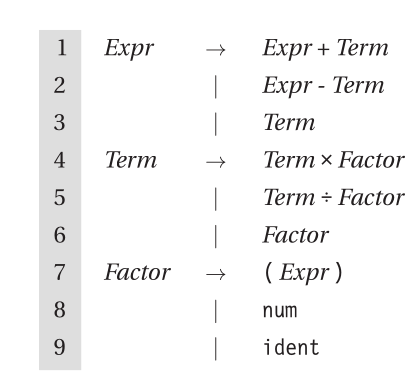
\includegraphics[width=\textwidth]{img/cfg.png}
               \caption{classic grammar for arithmetic expressions}
           \end{figure}
       \end{column}
       \begin{column}{0.6\textwidth}
        \begin{figure}
            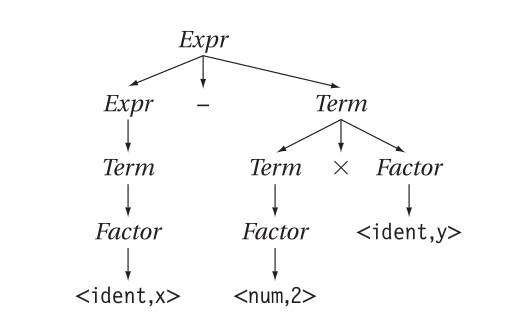
\includegraphics[width=\textwidth]{img/parse.png}
            \caption{parse tree for the expression x-2*y}
        \end{figure}
           
       \end{column}
   \end{columns}
\end{frame}
\begin{frame}
    \frametitle{Parsing techniques}
    Two main techniques:
    \begin{itemize}
        \item Top Down (recursive descent)
        
        Builds the parse tree from root to leaves. 
        Can be modified to do predicitve parsing (LL(1) parser).
        \item Bottom Up
        
        LR(1) parsers, build the parse tree from leaves to root. Bottom-up parsing handles a larger set of
        grammars
    \end{itemize}
   
    \textbf{We will focus on top down parsers.}
\end{frame}
\begin{frame}
    \frametitle{Top down parsers}
    \begin{block}{}Start from root of parse tree \end{block}
    \begin{block}{}At each level pick a production to match the input\end{block}
    \begin{block}{}If the derivation doesn't match the input $\Rightarrow$ backtrack and pick a different production\end{block}
\end{frame}